%%%%%%%%%%%%%%%%%%%%%%%%%%%%%%%%%%%%%%%%%
% Beamer Presentation
% LaTeX Template
% Version 1.0 (10/11/12)
%
% This template has been downloaded from:
% http://www.LaTeXTemplates.com
%
% License:
% CC BY-NC-SA 3.0 (http://creativecommons.org/licenses/by-nc-sa/3.0/)
%
%%%%%%%%%%%%%%%%%%%%%%%%%%%%%%%%%%%%%%%%%

%----------------------------------------------------------------------------------------
%	PACKAGES AND THEMES
%----------------------------------------------------------------------------------------

\documentclass{beamer}

\mode<presentation> {

% The Beamer class comes with a number of default slide themes
% which change the colors and layouts of slides. Below this is a list
% of all the themes, uncomment each in turn to see what they look like.

%\usetheme{default}
%\usetheme{AnnArbor}
%\usetheme{Antibes}
%\usetheme{Bergen}
%\usetheme{Berkeley}
%\usetheme{Berlin}
%\usetheme{Boadilla}
%\usetheme{CambridgeUS}
%\usetheme{Copenhagen}
%\usetheme{Darmstadt}
%\usetheme{Dresden}
%\usetheme{Frankfurt}
%\usetheme{Goettingen}
%\usetheme{Hannover}
%\usetheme{Ilmenau}
%\usetheme{JuanLesPins}
%\usetheme{Luebeck}
\usetheme{Madrid}
%\usetheme{Malmoe}
%\usetheme{Marburg}
%\usetheme{Montpellier}
%\usetheme{PaloAlto}
%\usetheme{Pittsburgh}
%\usetheme{Rochester}
%\usetheme{Singapore}
%\usetheme{Szeged}
%\usetheme{Warsaw}

% As well as themes, the Beamer class has a number of color themes
% for any slide theme. Uncomment each of these in turn to see how it
% changes the colors of your current slide theme.

%\usecolortheme{albatross}
%\usecolortheme{beaver}
%\usecolortheme{beetle}
%\usecolortheme{crane}
%\usecolortheme{dolphin}
%\usecolortheme{dove}
%\usecolortheme{fly}
%\usecolortheme{lily}
%\usecolortheme{orchid}
%\usecolortheme{rose}
%\usecolortheme{seagull}
%\usecolortheme{seahorse}
%\usecolortheme{whale}
%\usecolortheme{wolverine}

%\setbeamertemplate{footline} % To remove the footer line in all slides uncomment this line
%\setbeamertemplate{footline}[page number] % To replace the footer line in all slides with a simple slide count uncomment this line

%\setbeamertemplate{navigation symbols}{} % To remove the navigation symbols from the bottom of all slides uncomment this line
}

\usepackage{graphicx} % Allows including images
\usepackage{booktabs} % Allows the use of \toprule, \midrule and \bottomrule in tables

%----------------------------------------------------------------------------------------
%	TITLE PAGE
%----------------------------------------------------------------------------------------

\title[Python for finance]{Machine learning methods for stock return series analysis via Python} % The short title appears at the bottom of every slide, the full title is only on the title page
\author{Jian Wang } % Your name
\institute[Florida state university ] % Your institution as it will appear on the bottom of every slide, may be shorthand to save space
{Financial math Ph.D. candidate\\
\vspace{3ex}
Florida state university %%alifornia \\ % Your institution for the title page
\medskip
\textit{jwang@math.fsu.edu} % Your email address
}
\date{\today} % Date, can be changed to a custom date

\begin{document}

\begin{frame}
\titlepage % Print the title page as the first slide
\end{frame}

\begin{frame}
\frametitle{Overview} % Table of contents slide, comment this block out to remove it
\tableofcontents % Throughout your presentation, if you choose to use \section{} and \subsection{} commands, these will automatically be printed on this slide as an overview of your presentation
\end{frame}

%----------------------------------------------------------------------------------------
%	PRESENTATION SLIDES
%----------------------------------------------------------------------------------------

%------------------------------------------------
\section{Introduction} % Sections can be created in order to organize your presentation into discrete blocks, all sections and subsections are automatically printed in the table of contents as an overview of the talk
%------------------------------------------------

%\subsection{Subsection Example} % A subsection can be created just before a set of slides with a common theme to further break down your presentation into chunks

\begin{frame}
\frametitle{Introduction}
\begin{itemize}
\item \textbf{[Popular:]} Nowadays, Python becomes more and more popular in the financial
industry. For example, Bank of America Merrill Lynch and JP Morgan
Chase, use python to establish and enhance their core IT systems. In
the mean time, many of today's financial math engineering programs
use Python as one of the core languages for teaching the quantitative
finance knowledge into executable computer code.
\item  \textbf{[Reason:]}There are a couple of reasons that Python has had such recent
success. For example, it is an open source program language and its
ease of integration with almost any other technology.Beisdes, the computing speed for python is fast, so it is a powerful tool to handle the big data.
\item \textbf{[Purpose:]} In this project, we show that how to use python to analyze the financial data. Built machine learning models for stock return series. Compared the efficiency for language python and R. Finally, predict the future stock return based on the historical data.\\
\end{itemize}


\end{frame}

\section{DataSet}
\begin{frame}
\frametitle{Dataset}
The dataset is named stockdata which from huge package in R. It contained data that were
originally obtained from Yahoo! Finance. There are 1,258
observations representing 1,258 sequential trading days(form Jan 1 2003 to Jan 1 2008) and 452
variables, each of which was the day's closing share price for a different
stock within the Standard \& Poor's 500.We also add two index into the data set, one is S\&P 500 and another is Nasdaq(so totally 454 variables).\\
Among all the stock data , we used Goldman Sachs stock return
series as our response variable and other stocks as the predictors to analyze the stock return series movement.
\begin{columns}
\column{2.3in}
\textbf{Company:}:
 \begin{figure}
     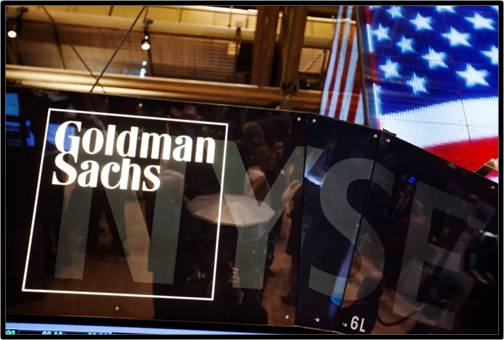
\includegraphics[width=0.6\textwidth, height=0.25\textheight]{gschart.jpg}
\end{figure}

\column{2.3in}

\textbf{Price:}:
\begin{figure}
     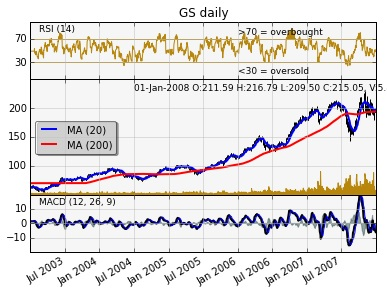
\includegraphics[width=0.6\textwidth, height=0.3\textheight]{gs_plot.jpg}
\end{figure}

\end{columns}
\end{frame}

\section{Methodology}

\begin{frame}
\frametitle{Methodology }

\setbeamercovered{transparent}
\begin{block}{Stock Return series}
\begin{equation}
R_t = ln( S_{t+1})-ln(S_t)
\end{equation}
Where $R_t$ is the stock return at trading day t and $S_t$ is the closing price of stock at trading day t.
\end{block}
\setbeamercovered{transparent}
\begin{block}{Ridge regression}
\begin{equation}
\hat{\beta}^{ridge}=argmin_{\beta}\{\sum_{i=1}^p{(y_i-\hat{y_i})^2}+{\color{red}\lambda \sum_{j=1}^p\beta_j^2}\}
\end{equation}
\end{block}

\begin{block}{Lasso regression}
\begin{equation}
\hat{\beta}^{lasso}=argmin_{\beta}\{\sum_{i=1}^p{(y_i-\hat{y_i})^2}+{\color{red}\lambda\sum_{j=1}^p \beta_j}\}
\end{equation}
\end{block}

\end{frame}


\begin{frame}
\frametitle{Methodology }
Comparison of L1 and L2 Penalized Model \\
\begin{columns}
\column{2.3in}
	\begin{block}{Ridge regression}
$\hat{\beta}^{ridge}=argmin_{\beta}\{\sum_{i=1}^p{(y_i-\hat{y_i})^2}+{\color{red}\lambda \sum_{j=1}^p\beta_j^2}\}$

\end{block}
\textbf{Coefficients}:
 \begin{figure}
     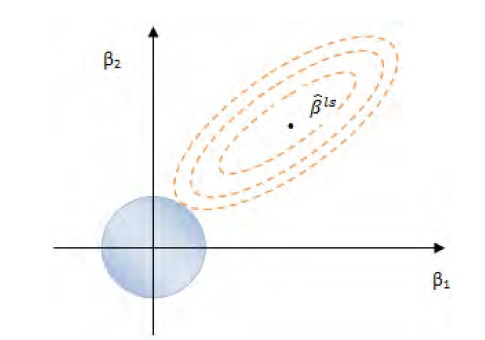
\includegraphics[width=0.9\textwidth, height=0.5\textheight]{ridge.jpg}

    \end{figure}

\column{2.3in}
\begin{block}{Lasso regression}

$\hat{\beta}^{lasso}=argmin_{\beta}\{\sum_{i=1}^p{(y_i-\hat{y_i})^2}+{\color{red}\lambda\sum_{j=1}^p \beta_j}\}$

\end{block}

\textbf{Coefficients}:
 \begin{figure}
     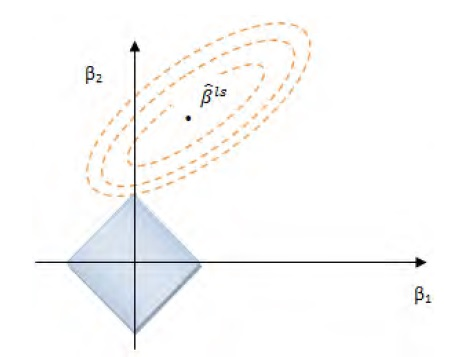
\includegraphics[width=0.9\textwidth, height=0.5\textheight]{lasso.jpg}

    \end{figure}
\end{columns}


\end{frame}

\begin{frame}
\frametitle{Methodology }
Comparison of L1 and L2 Penalized Model \\
\begin{columns}
\column{2.3in}
	\begin{block}{Ridge regression}
$\hat{\beta}^{ridge}=argmin_{\beta}\{\sum_{i=1}^p{(y_i-\hat{y_i})^2}+{\color{red}\lambda \sum_{j=1}^p\beta_j^2}\}$

\end{block}
\textbf{Path:}:
 \begin{figure}
     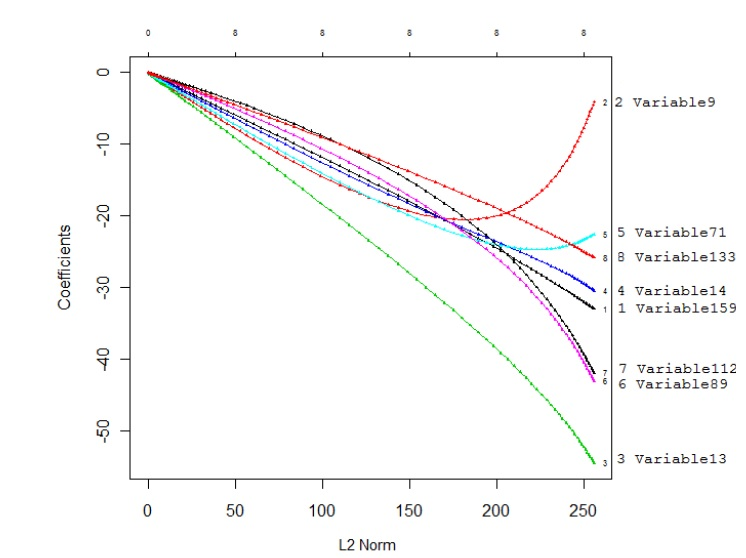
\includegraphics[width=0.9\textwidth, height=0.5\textheight]{ridge_p.jpg}

    \end{figure}

\column{2.3in}

\begin{block}{Lasso regression}

$\hat{\beta}^{lasso}=argmin_{\beta}\{\sum_{i=1}^p{(y_i-\hat{y_i})^2}+{\color{red}\lambda\sum_{j=1}^p \beta_j}\}$

\end{block}

\textbf{Path:}:
 \begin{figure}
     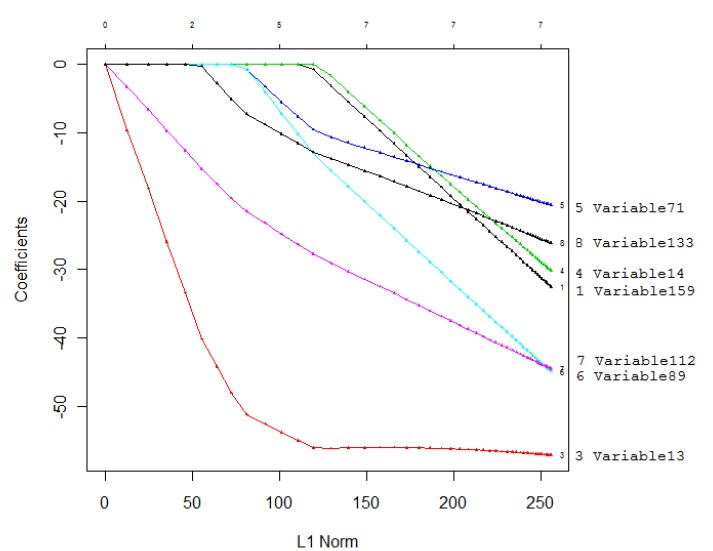
\includegraphics[width=0.9\textwidth, height=0.5\textheight]{lasso_p.jpg}

    \end{figure}
\end{columns}

\end{frame}

\begin{frame}
\frametitle{Methodology}
\setbeamercovered{transparent}
\begin{block}{Logistic Regression}
\begin{equation}
ln{\frac{F(x)}{1-F(x)}}=\beta_0+\sum_i\beta_ix_i
\end{equation}
\end{block}

\frametitle{Methodology}
\setbeamercovered{transparent}
\begin{block}{Support vector machine}
\begin{equation}
min{\sum_{i}[1-y_if]_{+}}+\frac{\lambda}{2}||\beta||
\end{equation}
\end{block}

\begin{columns}
\column{2.3in}
	 \begin{figure}
     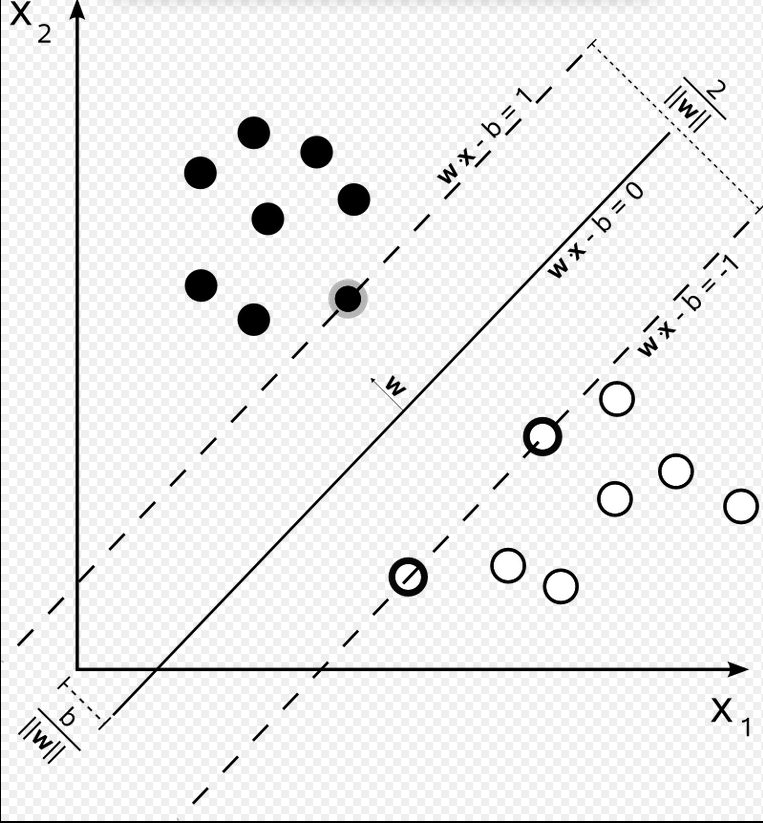
\includegraphics[width=0.6\textwidth, height=0.35\textheight]{svm.png}

    \end{figure}

\column{2.3in}
\textbf{Kernel Function:}\\
1) Linear\\
2) Polynomial\\
3) Radial basis\\
\end{columns}

\end{frame}


\begin{frame}
\frametitle{Methodology }
  \setbeamercovered{transparent}
  \begin{block}{Reference}
   \begin{itemize}
        \item  Tibshirani, R. (1996). "Regression shrinkage and selection via the lasso". Journal of the Royal Statistical Society, Series B 58 (1): 267–288. JSTOR 2346178
        \item Hoerl, A.E. and Kennard, R. (1970). Ridge regression: Biased
estimation for nonorthogonal problems. Technometrics, 12:
55-67
        \item Vapnik, V. (1995). "Support-vector networks". Machine Learning 20 (3): 273. doi:10.1007/BF00994018
    \end{itemize}
  \end{block}

  \begin{block}<2>{Packages}
    \begin{itemize}
        \item  R packages: glm, glmnet, e1071
        \item  Python packages: sklearn (svm, ridge, lasso, logistic)
    \end{itemize}
  \end{block}

\end{frame}


\section{Numerical results}

\begin{frame}
\frametitle{Numerical results}
\begin{itemize}
        \item  Python and R package comparison:\\
        we use the same day stock return series to compare the cpu time and accuracy date of the machine learning methods based on different languages(R and Python). Choose the first 1000 data as training data and the last remaining 257 data as testing. GS as response and the other 453 stocks as predictors.\\
        \item  Predict the stock data:\\
        we used the last one day, two day,... to five day stock returns as the predictors and today's
        GS return series as response to see if our model can be used to predict the stockdata.\\
        Still use the first 1000 data as training and the remaining 252 data as testing. GS as the response and the other 2270 variables as predictors.\\
    \end{itemize}

\end{frame}


\begin{frame}
\frametitle{Numerical results}
\begin{columns}
\column{2.3in}
	\begin{block}{CPU Time for R}
We changed the number of samples from 50 to 800, doubled each time to test the running time for the different machine learning methods:\\
\begin{figure}
     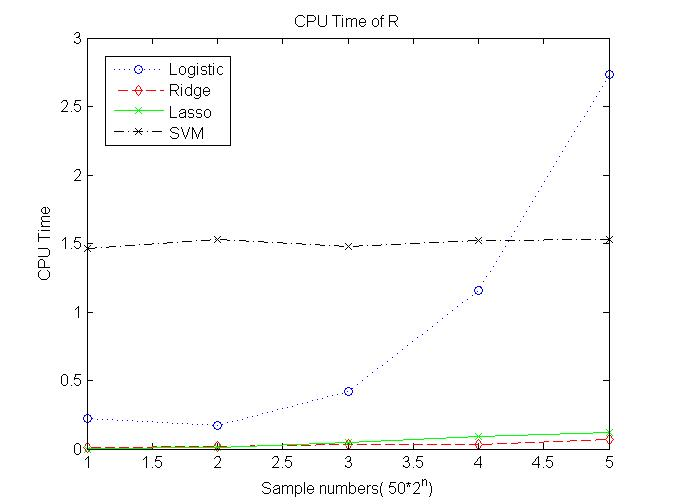
\includegraphics[width=0.8\textwidth, height=0.5\textheight]{cputime_r.jpg}

    \end{figure}

\end{block}

\column{2.3in}
\begin{block}{CPU Time for Python}
We changed the number of samples from 50 to 800, doubled each time to test the running time for the different machine learning methods:\\
\begin{figure}
     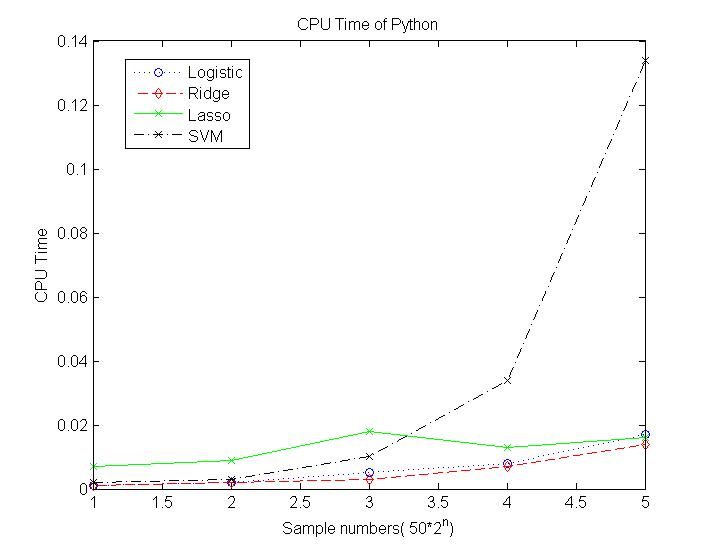
\includegraphics[width=0.8\textwidth, height=0.5\textheight]{cputime_python.jpg}

    \end{figure}
\end{block}

\end{columns}

\begin{block}{Results:}
Logistic and svm methods took long time than the other two in R , svm and lasso took long time in python.\\

\end{block}


\end{frame}

\begin{frame}
\frametitle{Numerical results}
\begin{block}{Comparison of CPU time for python and R }
\begin{center}
 \begin{figure}
     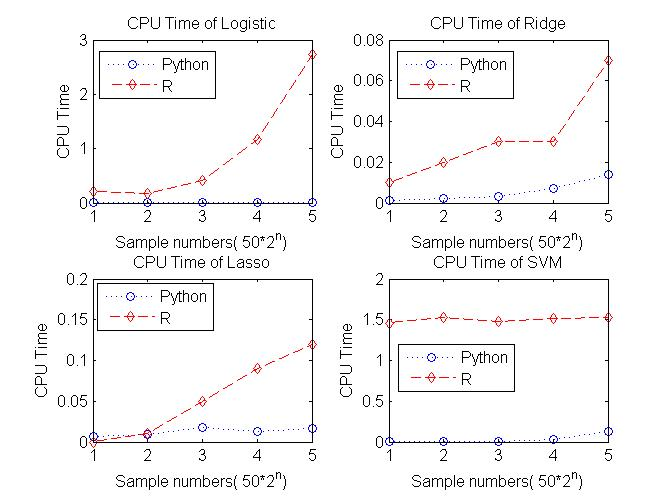
\includegraphics[width=0.8\textwidth, height=0.7\textheight]{cputime_python_r.jpg}

    \end{figure}
\end{center}
\end{block}

\begin{block}{Results:}
Python took smaller time for all the four methods compared with R.
\end{block}

\end{frame}

\begin{frame}
\frametitle{Numerical results:}

\begin{block}{Accuracy rate:}
\begin{table}[h!]\large
  \caption{Accuracy rate}
\begin{center}
    \begin{tabular}{| c | c| c | }
    \hline
    Methods& Python &  R\\
    \hline
Logistic  &77.8\%&	65.4\%\\
Ridge($\lambda$=1)&73.9\%	&77.4\%\\
Lasso($\lambda$=0.01)&78.6\%&	79.0\%\\
svm(linear)&72.4\%	&65.8\%\\
svm(poly)&74.3\%&	65.0\%\\
svm(rbf)&75.1\%	&72.8\%\\
\hline
\end{tabular}
\end{center}
\end{table}
\end{block}

\begin{block}{Results:}
\begin{itemize}
        \item  svm (rbf) and lasso ($\lambda$=0.01) performed better for both two languages.
        \item  Python performed better in most cases.
    \end{itemize}


\end{block}
\end{frame}


\begin{frame}
\frametitle{Numerical results:}
\begin{block}{Predicted}
\begin{equation}
R_t^{GS} = \sum_{i=1:5}{\sum_{j=1:454}\beta_{i,j}R_{t-i}^j}
\end{equation}
\end{block}

\begin{block}{Predict:}
\begin{table}[h!]\large
  \caption{Accuracy rate and CPU time}
\begin{center}
    \begin{tabular}{| c | c|c|}
    \hline
    Methods& Accuracy rate& CPU time \\
    \hline
Logistic  &51.2\%&0.1210\\
Ridge($\lambda$=1)&54.0\%&0.1230\\
Lasso($\lambda$=0.01)&49.2\%&0.0940\\
svm(linear)&52.8\%&1.1931\\
svm(poly)&45.6\%&1.2800	\\
svm(rbf)&47.2\%&1.2921\\
\hline
\end{tabular}
\end{center}
\end{table}

\end{block}

\end{frame}
%
%
\section{Future work}
\begin{frame}
\frametitle{Future work}
    \begin{itemize}
        \item  Compare with the time series model, such as Garch
        \item  Deal with the high frequency data instead of daily data
      \end{itemize}
\end{frame}

\section{Questions}
\begin{frame}
\frametitle{QA}
\begin{center}
\huge{Thanks a lot and Questions}
\end{center}
\end{frame}

%------------------------------------------------------------------

\end{document} 